\task{Дорога до метро}

\noindent Рассмотрим клетчатую сетку, её рёбра и узлы. Путём между двумя узлами будем называть последовательность рёбер, их соединяющую. Длину пути в разных случаях будем определять по-разному, однако стандартный способ~— понимать под длиной пути количество рёбер в нём.

\ms Определим {\itshape $k$--окрестность} узла — это множество всех узлов, до которых от данного существует путь длиной не более чем $k$. На рисунке M1 изображёны путь длины 3 и 3--окрестность центрального узла.

\begin{enumerate}

\item Длину пути можно ввести и по-другому. Давайте определим её как сумму величин смещения пути по горизонтали и по вертикали. Скажем, путь на рисунке M2 будет тогда иметь длину 5. Как будет выглядеть 4-окрестность фиксированного узла при так определёной длине?

\vspace{-0.3cm}
\begin{center}
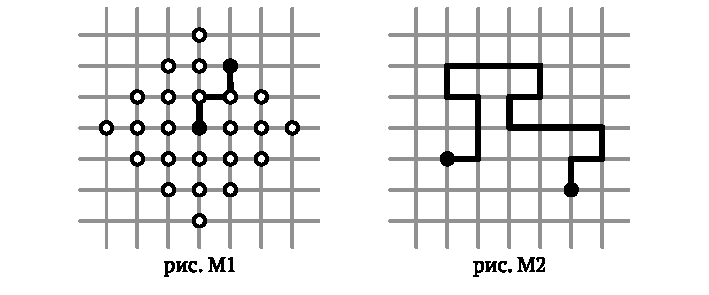
\includegraphics[width=10.5cm]{stats/2017/images/metro1.pdf}
\end{center} \vspace{-0.7cm}

\item А если мы определим длину пути как максимум\scolon как минимум\scolon как модуль разности величин смещения по горизонтали и по вертикали?

\item Рассмотрим два определения длины пути: стандартным способом и как в пункте 1. Понятно, что один путь может иметь разную длину в первом и во втором смысле. Докажите, тем не менее, что любая $k$--окрестность в смысле первой длины и в смысле второй длины выглядит одинаково.

\item Пусть длина пути определена стандартным образом. Пусть узел $B$ отстоит от узла $A$ на $m$ клеток вправо и на $n$ клеток вниз. Сколько кратчайших путей ведут из $A$ в $B$?

\end{enumerate}

\noindent Давайте теперь выберем из клетчатой сетки несколько узлов и некоторые рёбра между ними. Назовём выбранное нами {\itshape городом}. Расположим в каких-то из узлов города {\itshape станции метро}. Расстоянием от узла внутри города до данной станции метро будем называть длину (в стандартном смысле) кратчайшего пути между ними, лежащего внутри города. На рисунке M3 изображены пример города, пара станций метро, а также кратчайшие пути от одного из узлов до станций.

\begin{enumerate}

\item [5)] Для каждого узла в городе найдём ближайшую к нему станцию метро и расстояние до неё. Найдём в городе все узлы, в которых найденное расстояние достигает своего максимума. Теперь для каждого узла посчитаем сумму расстояний от него до всех станций метро и тоже найдём узлы, где эта сумма достигает максимального значения.

\smallskip\noindent Придумайте город и расстановку в нём станций метро такую, что множества узлов, где максимально кратчайшее расстояние, и узлов, где максимальна сумма расстояний, не пересекаются.

\vspace{-0.3cm}
\begin{center}
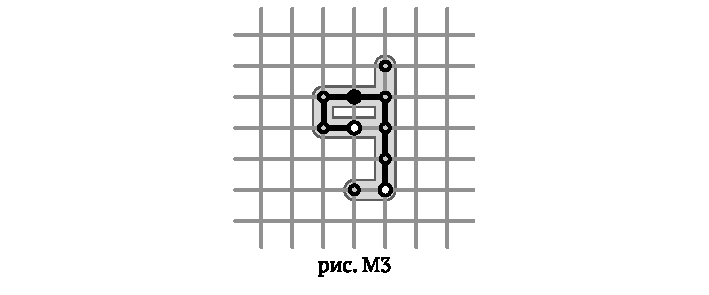
\includegraphics[width=10.5cm]{stats/2017/images/metro2.pdf}
\end{center} \vspace{-0.7cm}

\item[6)] Докажите, что какой бы ни была расстановка станций метро в произвольном городе, максимальная сумма расстояний и максимальное среднее расстояние до станций всегда достигаются в одних и тех же узлах.

\item[7)] Для каждого узла в городе найдём самую далёкую от него станцию метро и расстояние до неё. Найдём в городе все узлы, в которых найденное расстояние достигает своего максимума.

\smallskip\noindent Придумайте город и расстановку в нём станций метро такую, что три множества: узлов, где максимально кратчайшее расстояние\scolon узлов, где максимальна сумма расстояний\scolon узлов, где максимально наибольшее расстояние — не пересекаются.

\item[8)] Какие ещё особенные узлы можно рассматривать в городе со станциями метро?  Предложите свои направления исследования и изучите их.

\end{enumerate}